\chapter{簡介}
\section{情境}
根據美國能源資訊署（U.S. Energy Information
Administration, EIA）統計資料\cite{eia_ami_2024}......., 如圖 \ref{fig:AMI_count} 所示。
\\測試測試

\begin{figure}[!h]
    \centering
    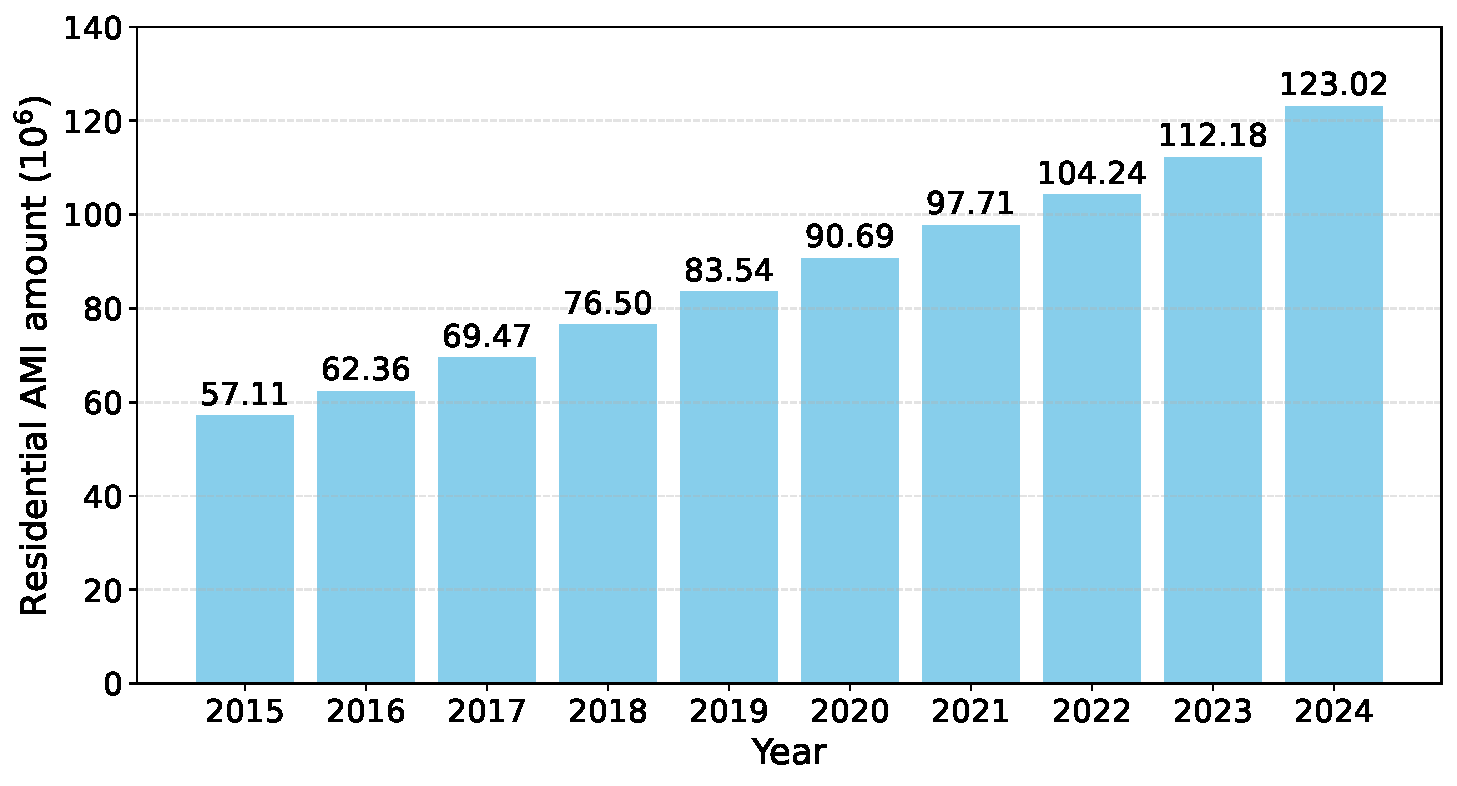
\includegraphics[width=\textwidth]{figures/AMI_count.pdf}
    \caption{美國住宅 AMI 智慧電表數量成長趨勢}
    \label{fig:AMI_count}
\end{figure}

\clearpage

\section{現況與問題討論}
\subsection{現況1}
\begin{itemize}
    \item 現況1.1
    \item 現況1.2
    \item 現況1.3
\end{itemize}

\subsection{現況2}
\begin{enumerate}
    \item 現況2.1
    \item 現況2.2
    \item 現況2.3
\end{enumerate}

{ \color{red} 要標示成紅色的文字1 }

\textcolor{red}{ 要標示成紅色的文字2 }

\redcolor{ 要標示成紅色的文字3 } % 自訂指令，不是latex內建

\bluecolor{ 要標示成藍色的文字3 } % 自訂指令，不是latex內建

\cyancolor{ 要標示成青色的文字3 } % 自訂指令，不是latex內建

\textbf{ 要標示成粗體的文字 }

\textit{ italic text } % 要標示成斜體的文字，限英文

\clearpage
並排插入2張圖片。Insert two pictures side by side.

% 並排插入2張圖片(獨立的2個圖標題)
\begin{figure}[!h]
  \centering
  \begin{minipage}[b]{0.49\textwidth}
    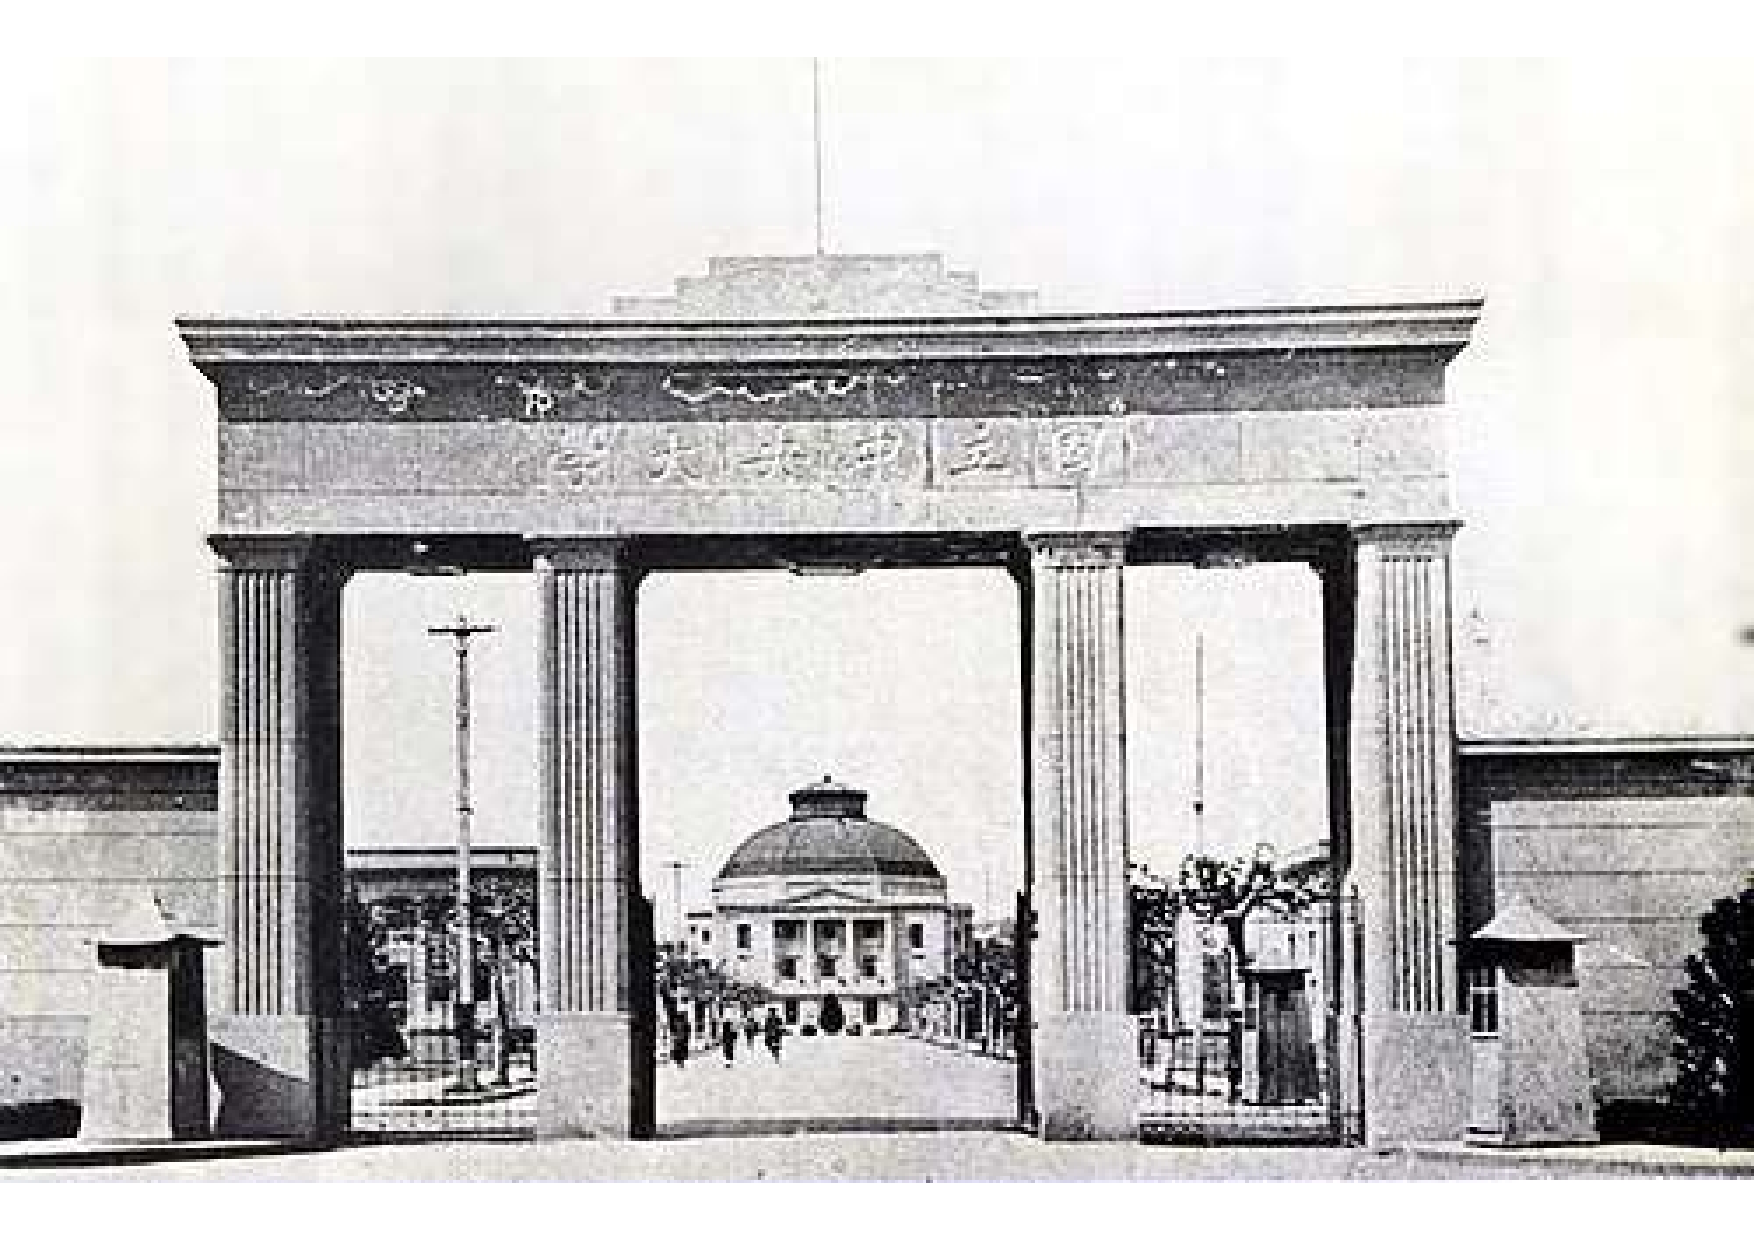
\includegraphics[width=\textwidth]{figures/南京國立中央大學正門.pdf}
    \caption{南京國立中央大學正門}
    \label{fig:bus_count}
  \end{minipage}
  \hfill
  \begin{minipage}[b]{0.49\textwidth}
    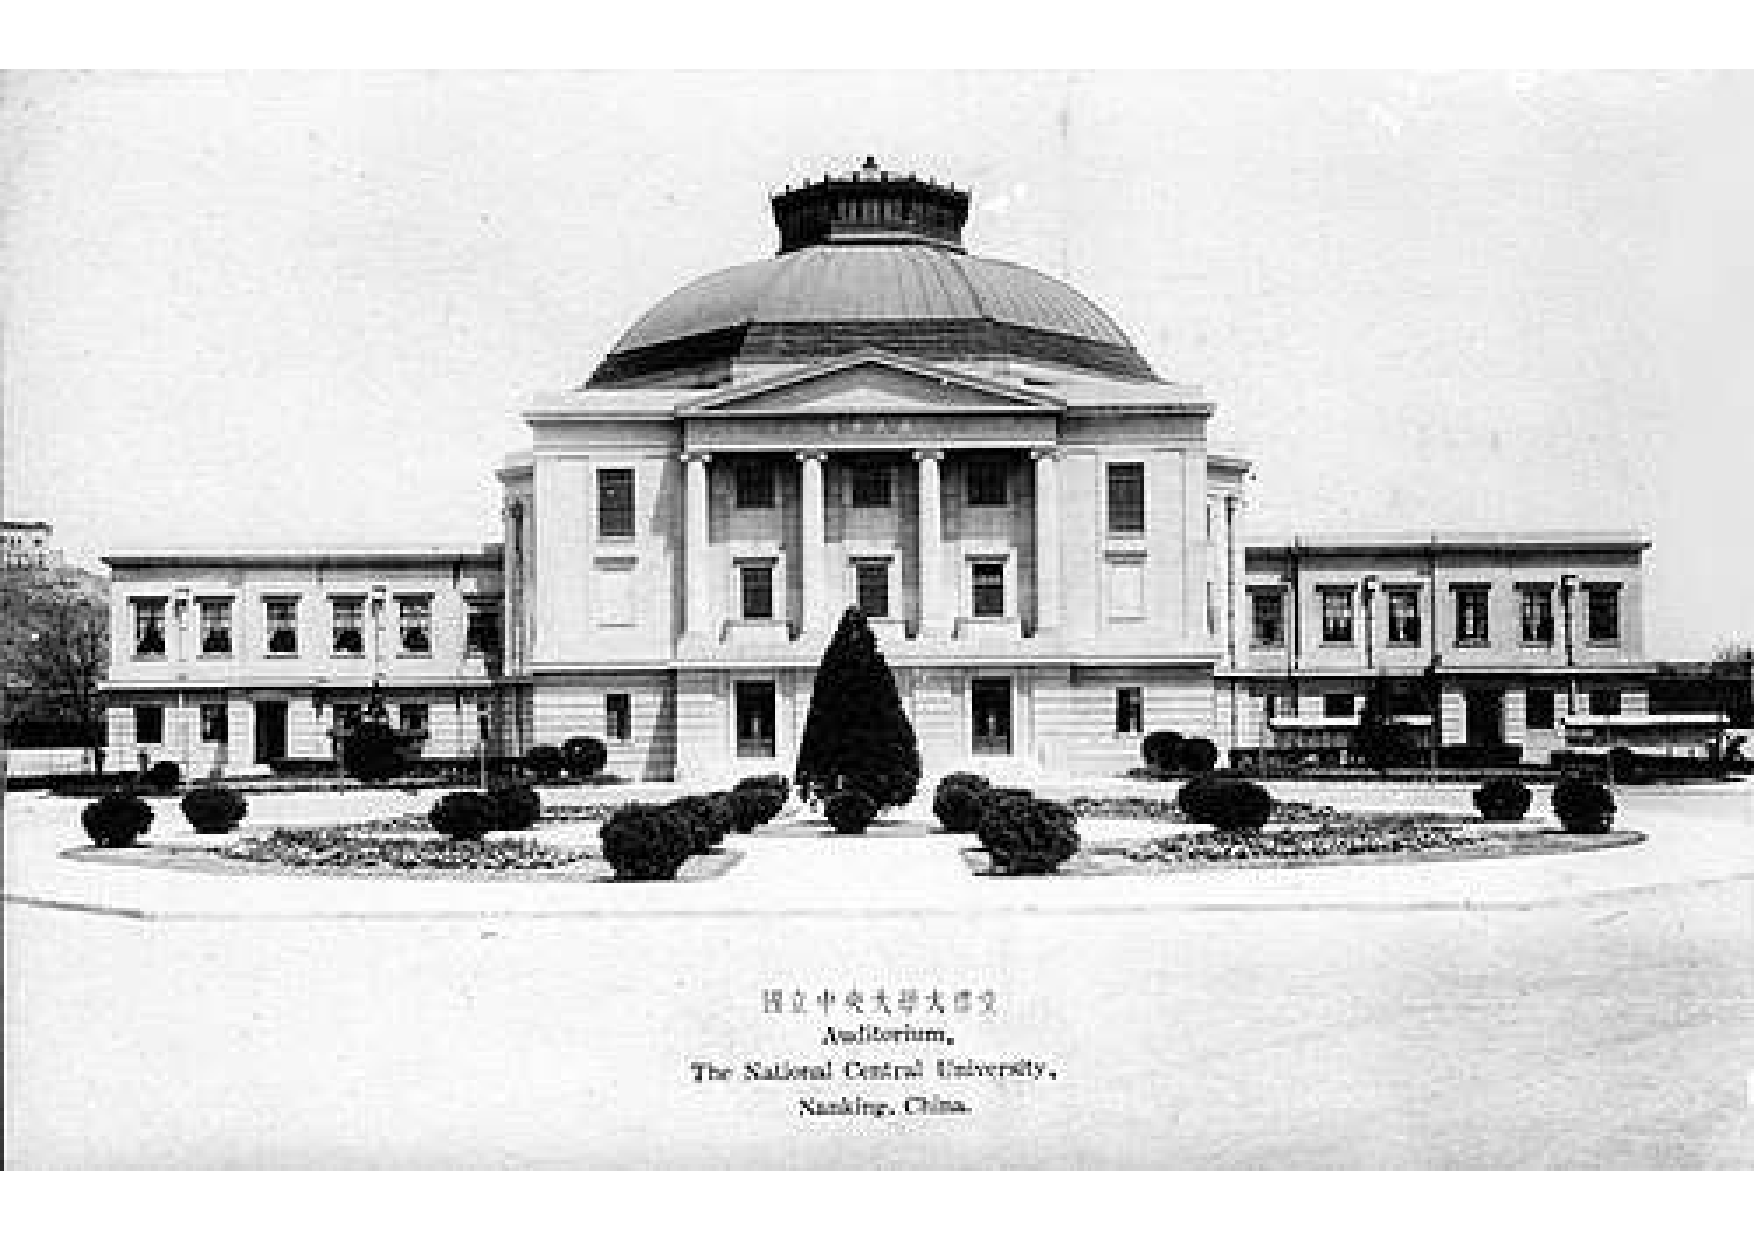
\includegraphics[width=\textwidth]{figures/南京國立中央大學大禮堂.pdf}
    \caption{南京國立中央大學大禮堂}
    \label{fig:new_bus_count}
  \end{minipage}
\end{figure}

% 並排插入2張圖片(1個圖標題，拆分為2個子標題a,b)
\begin{figure}[!h]
  \centering
  \subfigure[圖示1]{
  \label{fig:ami_count1}
  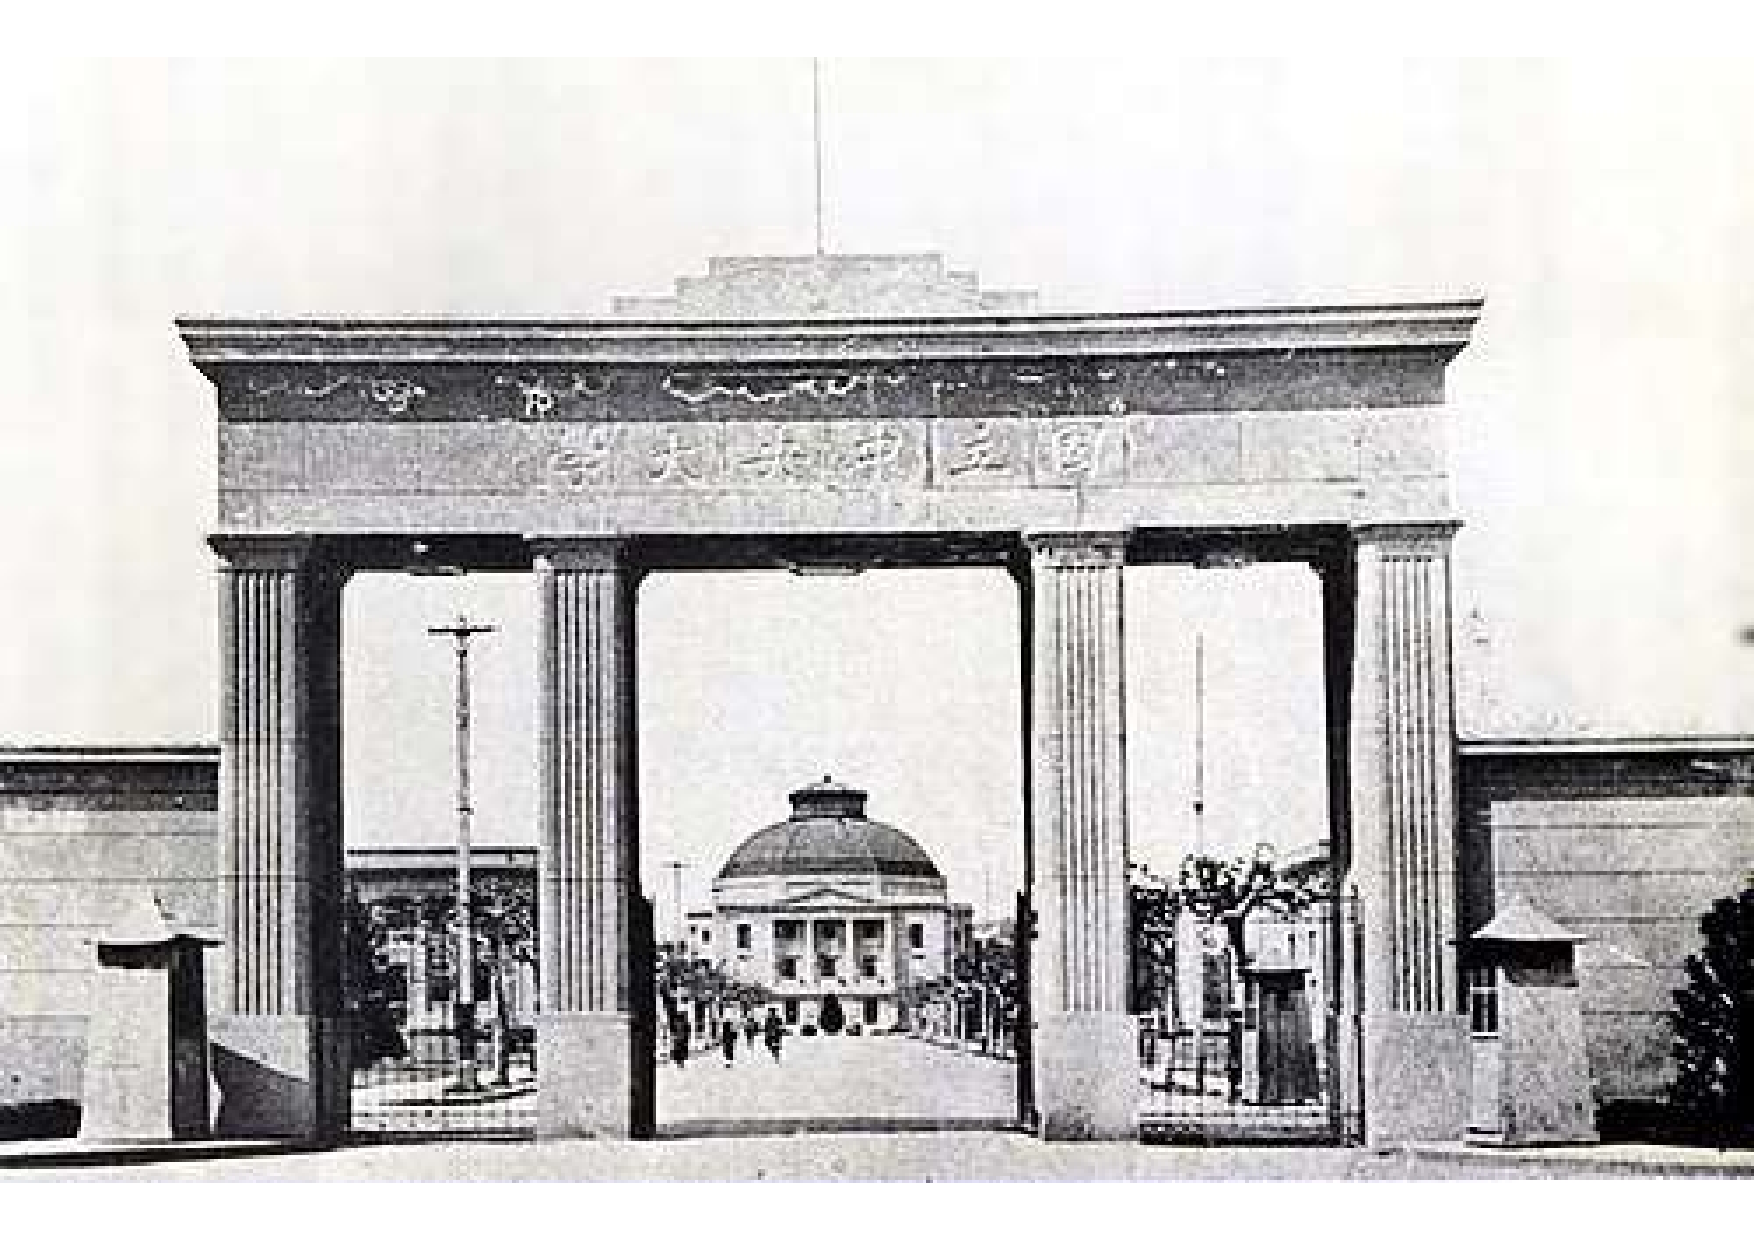
\includegraphics[width=0.49\textwidth]{figures/南京國立中央大學正門.pdf}}
  \subfigure[圖示2]{
  \label{fig:ami_count2}
  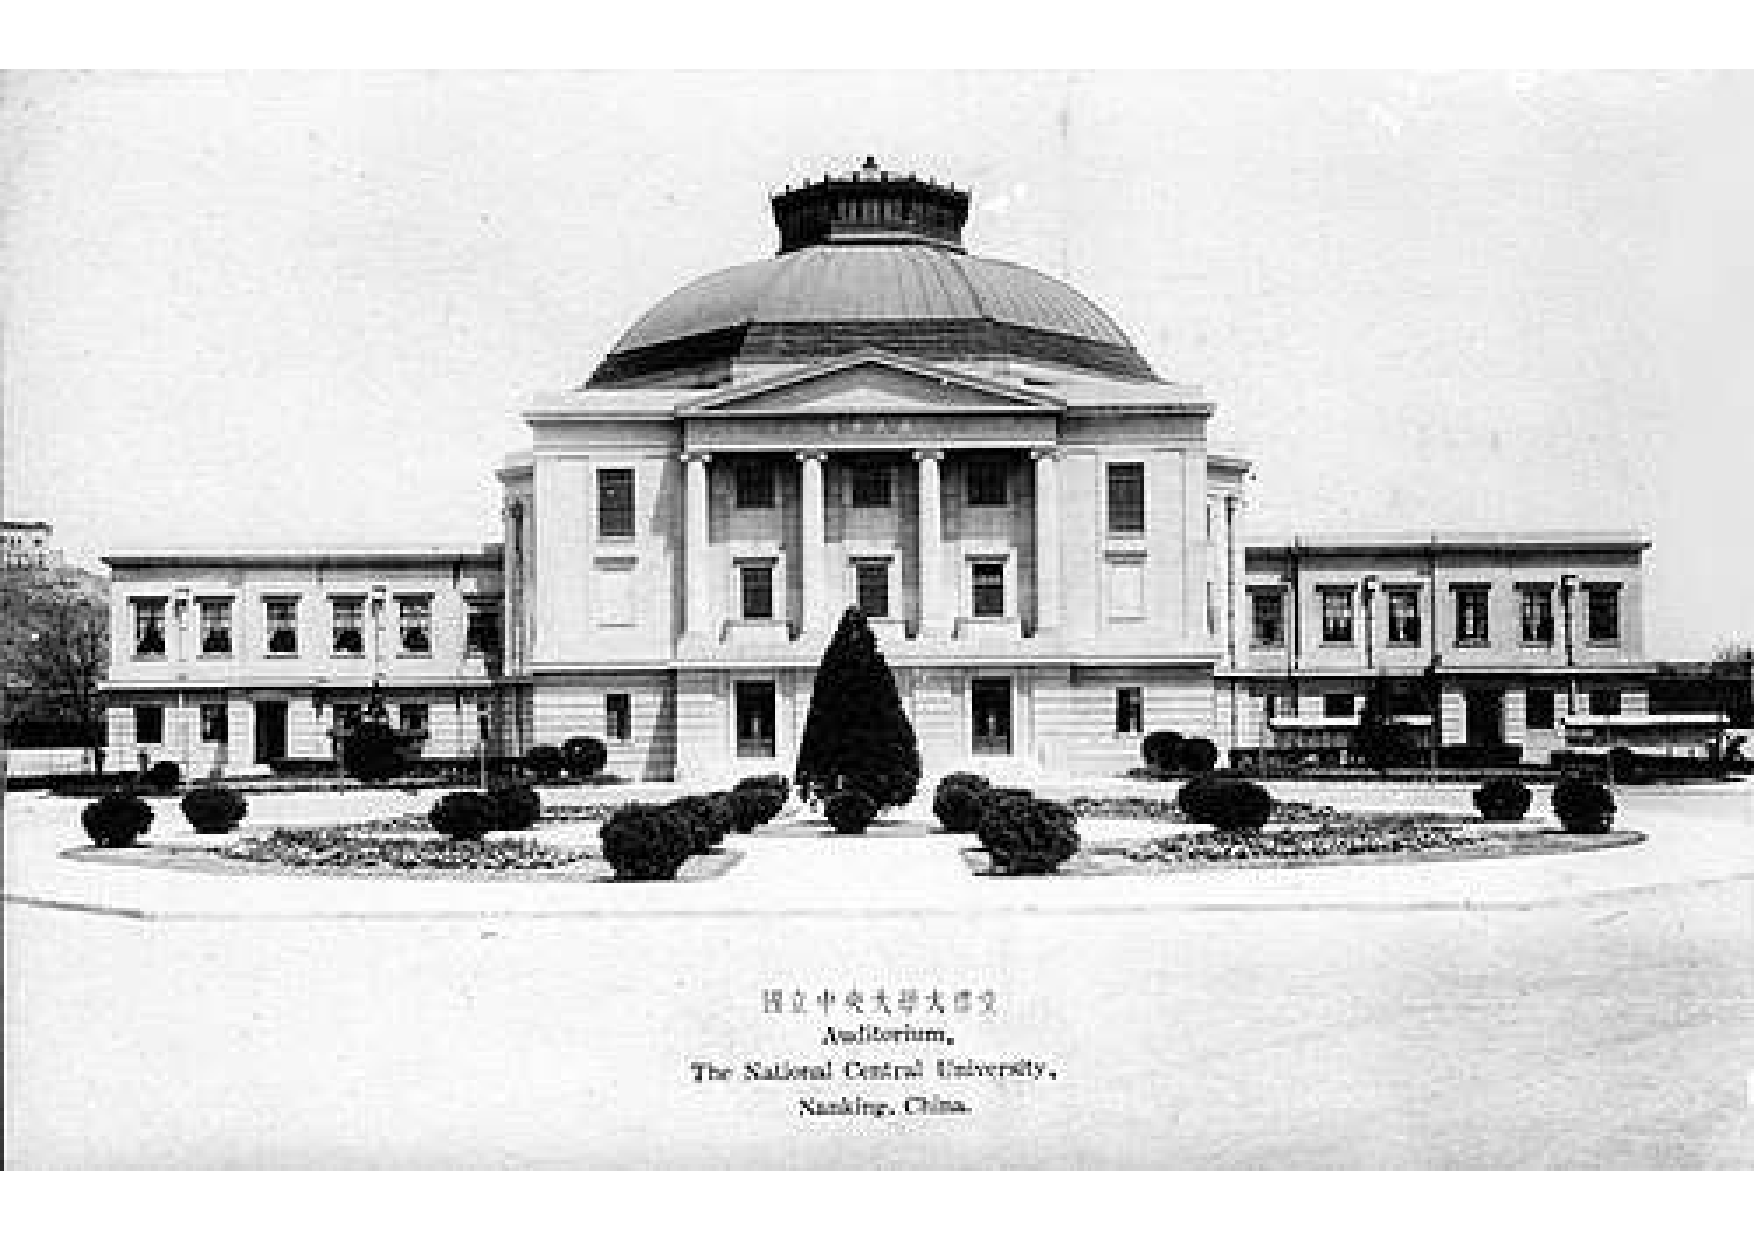
\includegraphics[width=0.49\textwidth]{figures/南京國立中央大學大禮堂.pdf}}
  \caption{南京國立中央大學校景}
  \label{fig:ami_count3}
\end{figure}

\clearpage

\subsection{現況3}
% 表格
\begin{table}[!h]
    \centering
    \caption{電動車軌跡記錄範例}
    \vspace{6pt}
    \begin{tabular}{|c|c|c|c|c|c|}
    \hline
        車號 & 日期 & 時間 & 經度 & 緯度 & 速度 \\\hline
        EXX-XXXX & 2026/11/14 & 14:00 & 120.6708 & 24.1482 & 50 \\\hline
        EXX-XXXX & 2026/11/15 & 14:35 & 120.6755 & 24.1512 & 65 \\\hline
    \end{tabular}
    \label{tab:ev_location_record_sample}
\end{table}

國立中央大學，官方簡稱中大，是位於臺灣桃園市中壢區的一所公立研究型大學。因創校於中華民國首都南京市而得名中央，其前身甚多，1928年5月定名為國立中央大學。1962年經戴運軌等校友籌備努力在臺復校，1967年由苗栗縣遷入現址。

中大前身為創立於1915年的國立南京高等師範學校。由表\ref{tab:ev_location_record_sample}
\\斜線*2或空一行就可以分段。


\begin{figure}[!h]
    \centering
    
\includegraphics[width=0.5\linewidth]{figures/NCU_logo.jpg}
    \caption{國立中央大學校徽}
    \label{fig:enter-label}
\end{figure}

\vspace{1\baselineskip}  % 垂直空出「1行」的高度
智慧家庭與物聯網根據 \cite{li2025bigdata}，

\vspace{1\baselineskip}  % 垂直空出「1行」的高度
%%%%%%%%%%%%%%%%%%%%%%%%
\begin{equation}
\ f(x) =
\int (2x^3 - x)\,dx = \frac{2}{4}x^4 - \frac{1}{2}x^2 + C = \frac{1}{2}x^4 - \frac{1}{2}x^2 + C
\end{equation}

\begin{equation}
f(x) = \int (2x^3 - x)\,dx 
= \frac{2}{4}x^4 - \frac{1}{2}x^2 + C 
= \frac{1}{2}x^4 - \frac{1}{2}x^2 + C
\end{equation}

\begin{align}
f(x) &= \int (2x^3 - x)\,dx \notag \\
     &= \frac{2}{4}x^4 - \frac{1}{2}x^2 + C \notag \\
     &= \frac{1}{2}x^4 - \frac{1}{2}x^2 + C
\end{align}


\bigskip % 插入約12pt高度的垂直空白
以下是DQN的pseudocodez範例:
\begin{algorithm}
\caption{Double Q-learning}
\begin{algorithmic}[1]
\STATE Initialize $Q^A, Q^B, s$
\REPEAT
    \STATE Choose $a$ based on $Q^A(s, \cdot)$ and $Q^B(s, \cdot)$, observe $r, s'$
    \STATE Choose (e.g. random) either UPDATE(A) or UPDATE(B)
    \IF{UPDATE(A)}
        \STATE Define $a^* = \arg\max_{a} Q^A(s', a)$
        \STATE $Q^A(s, a) \leftarrow Q^A(s, a) + \alpha(s, a)\left[r + \gamma Q^B(s', a^*) - Q^A(s, a)\right]$
    \ELSIF{UPDATE(B)}
        \STATE Define $b^* = \arg\max_{a} Q^B(s', a)$
        \STATE $Q^B(s, a) \leftarrow Q^B(s, a) + \alpha(s, a)\left[r + \gamma Q^A(s', b^*) - Q^B(s, a)\right]$
    \ENDIF
    \STATE $s \leftarrow s'$
\UNTIL{end}
\end{algorithmic}
\end{algorithm}
